The allocation sequence ended with a measured paradox: the corrected
allocator could deliver candidate substrate (permanence supply tripled),
and yet the second block's protected structure stayed at \(\approx
1/10\) of the first block's mass. The resolution required decomposing
what a newly consolidated synapse needs \emph{after} permanence: LTP
support from co-firing postsynaptic activity. Two read-only audits
\cite{wgrowth,drive}, both over the committed source-correction runs
(registration-era baselines of \S\ref{sec:rg}), localized the failure
to the very first link of the second block.

\subsection{Event-level decomposition (weight-growth audit)}

For the 61 C-cohort permanence events of the second block in the
baseline blocked run, the per-synapse decomposition is complete
\cite{wgrowth}:

\begin{itemize}
\item starting weight at permanence: \(w_{\mathrm{c,perm}}=0.02\)
(snapshot-verified);
\item pre-spikes: abundant --- C channels fire 56--87 spikes per
500 ms presentation; the input side is not starved;
\item post-spikes: the decisive deficit --- the last A presentation
fires 1{,}697 internal spikes; the first C presentation fires 101;
C presentations sustain 101--222 (a 17\(\times\) collapse at the
block switch; A-block presentations run 1{,}300--1{,}700);
\item applied LTP: the STDP balance on the C cohort over the C block is
\emph{net negative} (\(-21.63\) over 1{,}961 coalesced events): with
post activity so sparse, the dominant pre/post pairing is LTD;
\item per-synapse growth is intact whenever posts exist (measured
factors of 2.5--3.8\(\times\), e.g.\ \(0.02 \to 0.185\));
\item M2 is not suppressing: the working target stays
0.360 \(\to\) 0.303 across the block (per-neuron \(P\)
0.44 \(\to\) 0.50, cap 0.60);
\item M4 is quiet in the second block: 23 C-afferent prunes vs.\ 161 in
the first block;
\item causal order: the post-activity collapse (pres-21) precedes every
C permanence (first at \(t=47{,}500\), 2.5 s after onset) and all C
weight growth.
\end{itemize}

Verdict: \textbf{event-limited (A)} --- second-block C fails at the
level of relevant postsynaptic LTP opportunities; the growth machinery
works where posts exist.

\subsection{Drive decomposition and the IL control (drive audit)}

Why do C presentations produce a hundred spikes instead of a thousand?
The drive audit \cite{drive} decomposed the first-exposure currents
(per-neuron means, snapshot + spike telemetry):

\begin{center}
\footnotesize
\begin{tabular}{lcc}
\toprule
quantity (first exposure, per neuron) & first-A (block 1, pres 1) & first-C (block 2, pres 21) \\
\midrule
afferent current \(I_{\mathrm{aff}}\) & 11.98 & 1.57 \\
recurrent current \(I_{\mathrm{rec}}\) & 6.90 & 0.05 \\
inhibitory current \(I_{\mathrm{inh}}\) & \(-2.19\) & \(-0.81\) \\
posts/n & 0.98 & 0.12 \\
\bottomrule
\end{tabular}
\end{center}

The first-C presentation delivers \(\approx 7.7\times\) less afferent
current than the first-A presentation did, all of it working
(unconsolidated): block-1 churn (M2 working-budget squeeze + M4
pruning, dominated by passive decay per SDE-C2) reduced the live C
working afferents from \(\approx 197\) to \(\approx 29\) before C was
ever presented. With 1.6 drive/neuron and no recurrent support, the
population sits below threshold; no posts; no recurrent bootstrap; the
LTD-dominant STDP balance; protected structure starves. M6 inhibition is
excluded as the cause: it is 2.7\(\times\) \emph{lower} at first C than
at first A (it follows activity, it does not create the deficit).

The control that converts this from correlation to causation is the
interleaved regime. In the committed alternating runs, C is present
from presentation 1, so its substrate is never churned; first-C
afferent current is 11.13/neuron, recurrent 7.05, posts 1.00 ---
numerically identical to A's first contact --- and C permanence (98)
matches A (95) \cite{drive}. The blocked-vs-alternating comparison
isolates \emph{prior representation / substrate competition} as the
variable: the C stimulus itself is intrinsically fine.

\begin{quote}
\textbf{Demonstrated:} first-exposure drive for a late pattern is
\(\approx 8\times\) below first-block levels because its working
substrate was destroyed before exposure (prunes +18--31\%; passive
decay family per SDE-C2); posts collapse 17\(\times\); the mechanism is
event-limited, not LTP-, M2-, or M4-limited.\\[1pt]
\textbf{Supported:} the deficit is curriculum-inherent (blocked-order
churn); the alternating regime recruits symmetrically without any
added mechanism.
\end{quote}

\begin{figure}[t]
\centering
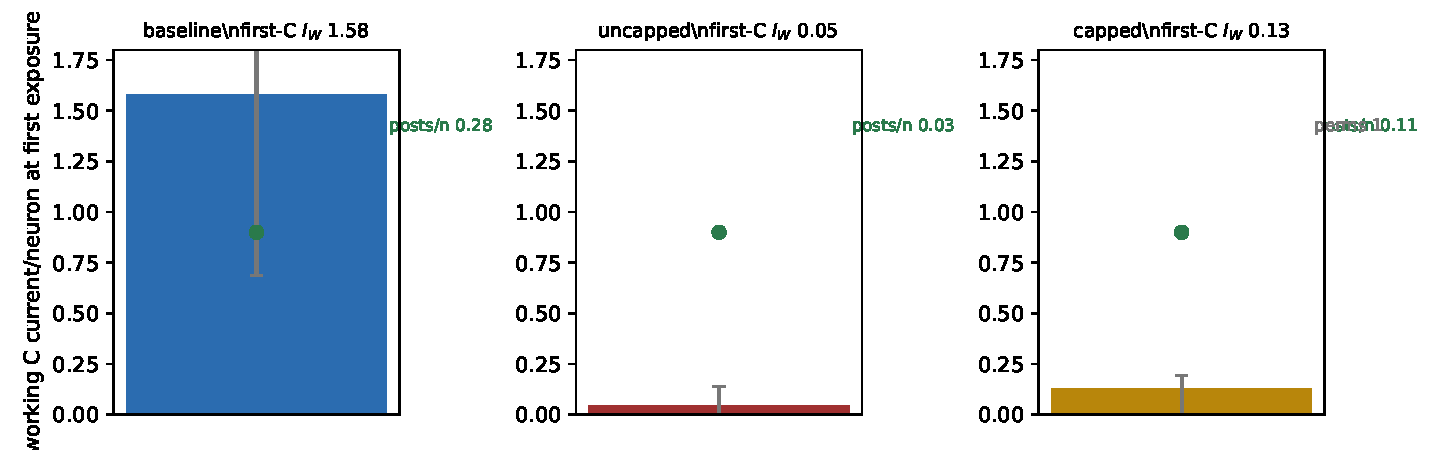
\includegraphics[width=\linewidth]{figures/fig7-decomp.pdf}
\caption{\textbf{Allocation/recruitment failure decomposition} at first
exposure of the late pattern (blocked runs, three seeds; bars show
mean over seeds, ticks the range). Left: working afferent current
surviving to first exposure (baseline 1.565/neuron) collapses under the
uncapped gain and is only partially rescued by the cap. Center: first-
exposure posts/n. Right: second-block permanence events (bar 150).
All panels from preserved runs via the committed \texttt{rg8eval}
instrument \cite{rg8,rg8c}.}
\label{fig:decomp}
\end{figure}